\section{Implementação dos métodos}\label{cap:artefato}

\subsection{Versão e fluxo efetivo}

A versão atual examinada é \texttt{GK-P2.1-dev}, com regra comum nos quatro chats e duas instruções de linguagem. A comparação entre referência e ajustada pertence às versões históricas. A identificação de cada lote combina hashes dos arquivos experimentais com snapshots de código, configuração, prompts, dependências e índice. Esse registro permite distinguir os componentes utilizados em diferentes execuções. O piloto histórico é apresentado separadamente no Capítulo~\ref{cap:evidencias}.

A Figura~\ref{fig:arquitetura} organiza a arquitetura em duas camadas: entrada, recuperação e geração; verificação e entrega. As molduras tracejadas agrupam funções, e as setas indicam a sequência do caminho completo. Encerramentos alternativos são detalhados na Figura~\ref{fig:decisao}. Antes de inferência há validação de entrada e uma detecção local parcial de identificadores pessoais. O classificador de entrada produz categoria, necessidade de proteção, predação educativa, busca de ajuda e justificativa. Proteção tem precedência sobre a exceção educativa. Quando a entrada prossegue, a busca fornece até três passagens acima do limiar. Ausência de passagens provoca redirecionamento, não demonstra ausência real de apoio.

\begin{figure}[htbp]\centering
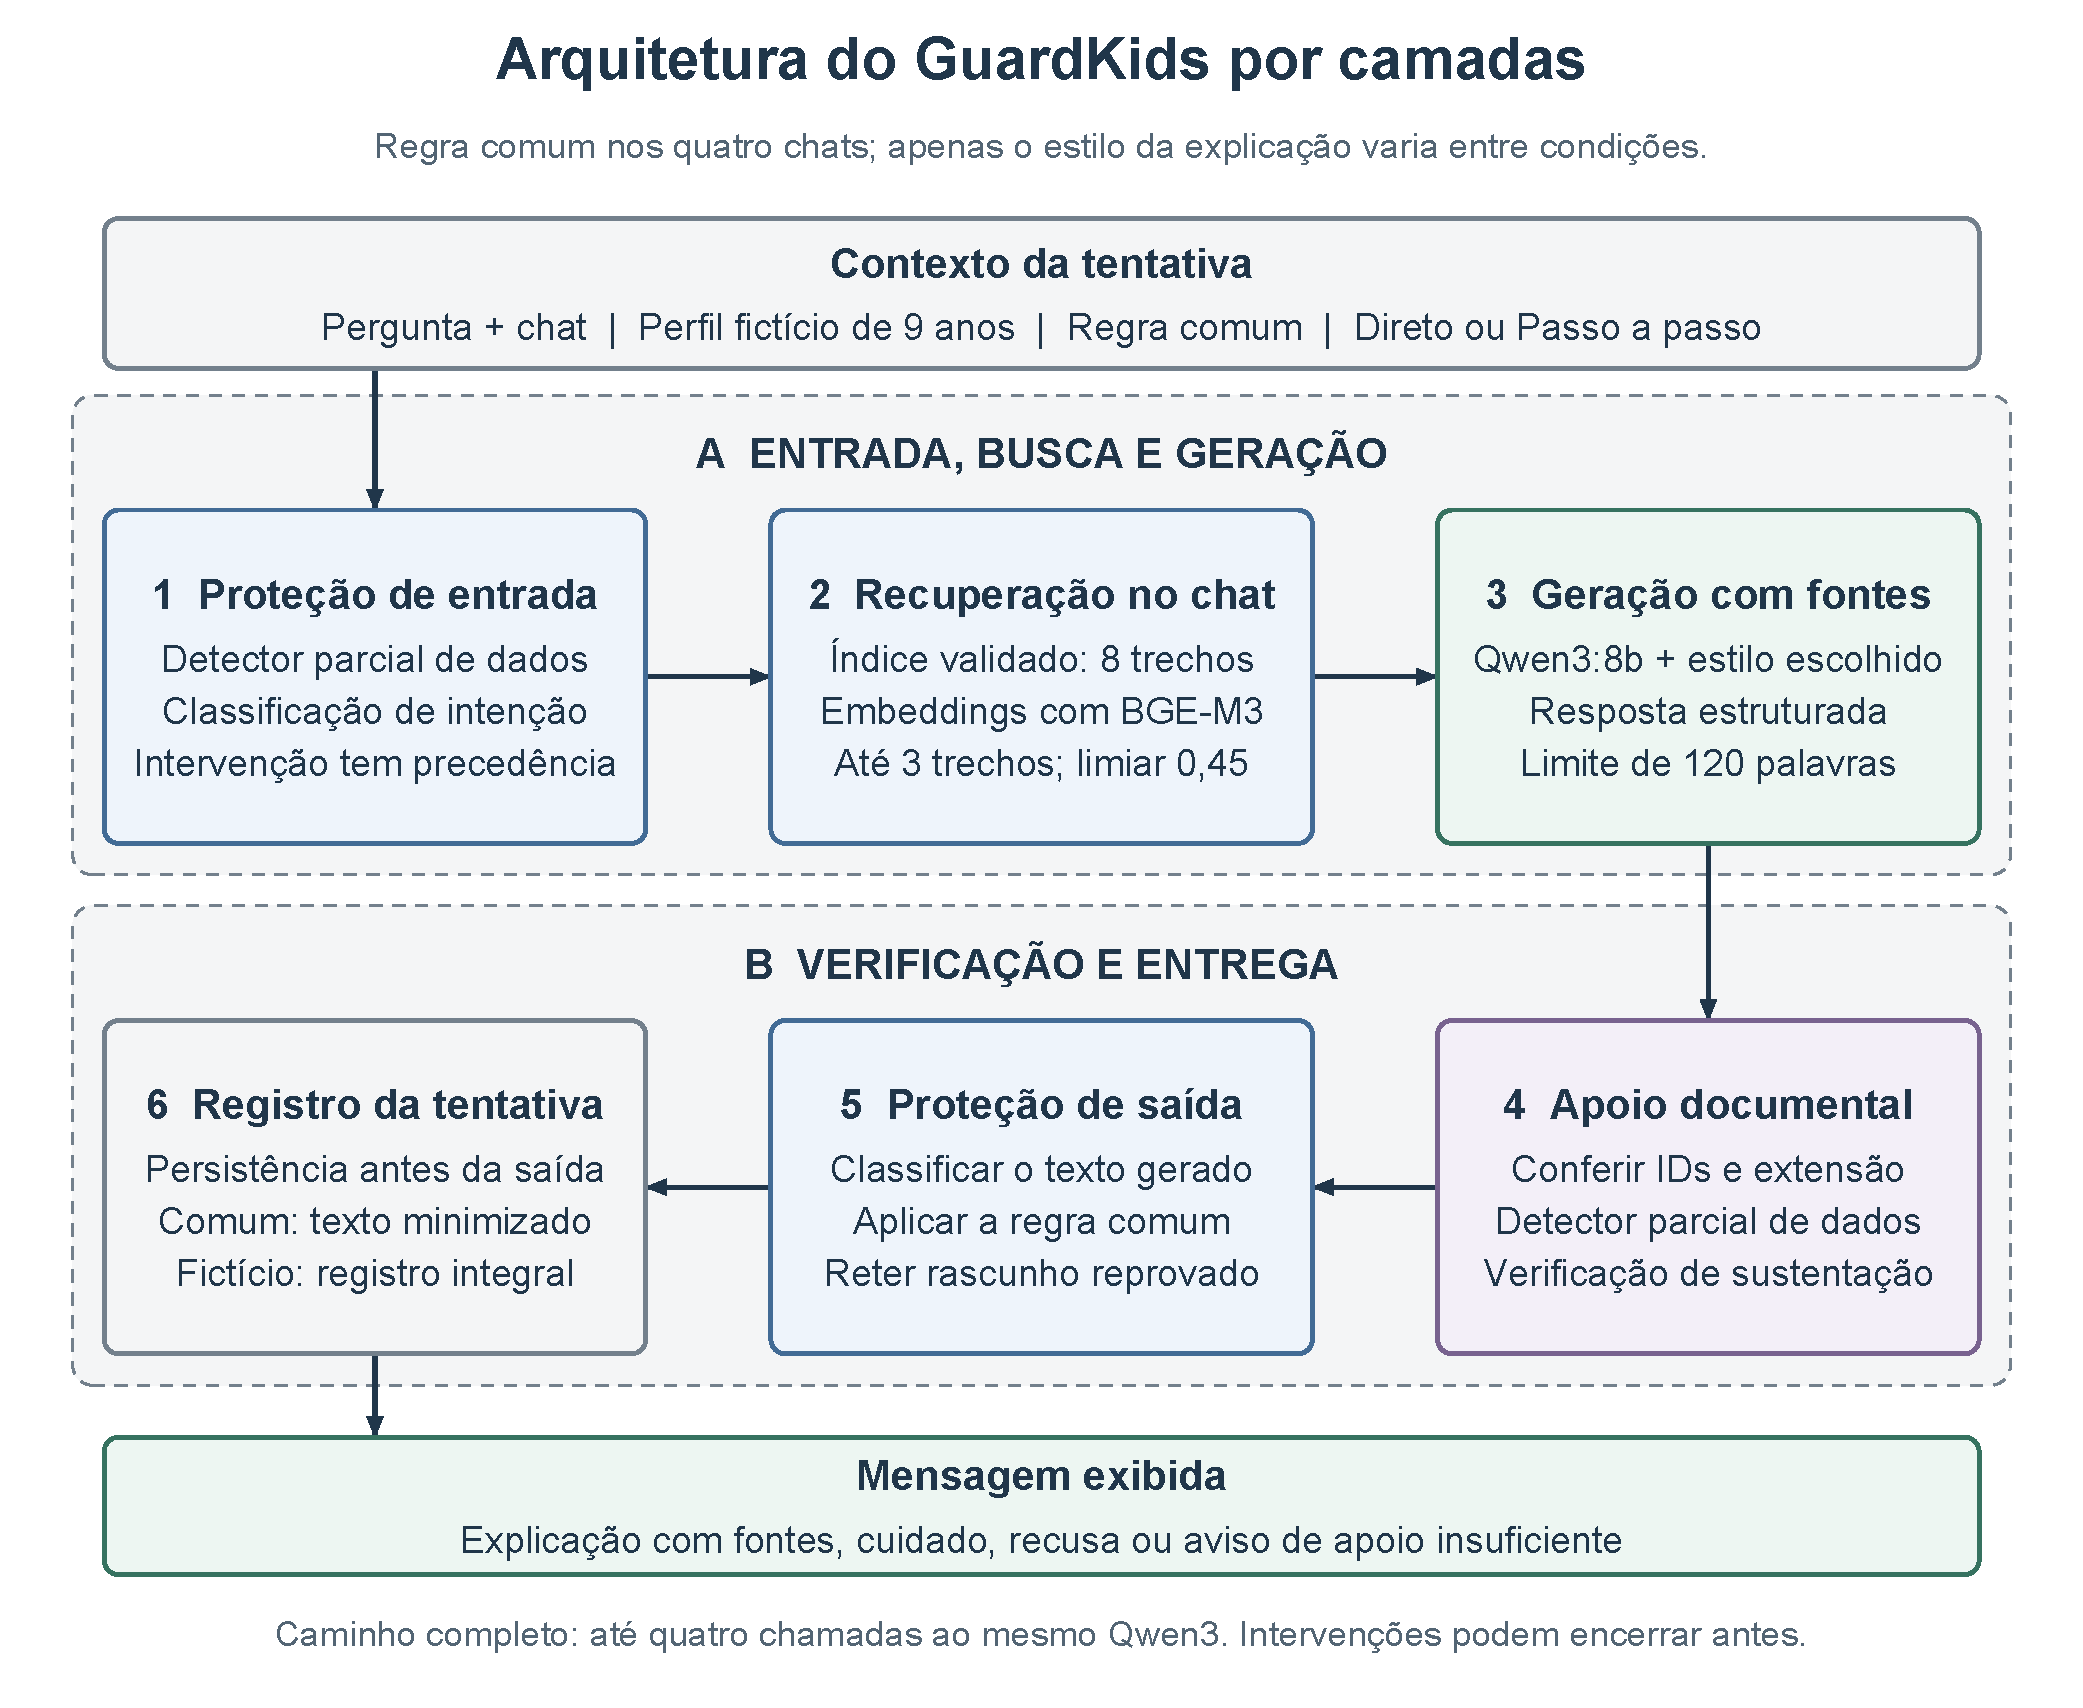
\includegraphics[width=\textwidth]{diagramas/pdf/03_arquitetura_conceitual_integrada.pdf}

\caption{Arquitetura em camadas e caminho completo da PoC}\label{fig:arquitetura}
\fonte{Elaboração própria a partir da implementação do protótipo.}
\end{figure}

O gerador informa resposta, IDs de fontes e indicação de apoio. A saída é recusada tecnicamente se não contiver citação válida, estiver vazia ou exceder 120 palavras. Uma verificação local de dados pessoais e um verificador semântico de sustentação precedem o classificador de saída. Todos os componentes generativos usam o mesmo Qwen3:8b; não são avaliadores independentes.

No caminho completo há \textbf{quatro chamadas ao LLM}: classificação de entrada, geração, sustentação e classificação de saída, além de uma chamada de embedding da pergunta. Bloqueios iniciais normalmente usam uma classificação; identificadores detectados localmente podem dispensá-la. A falta de passagens encerra após classificação e embedding; insuficiência declarada pelo gerador e reprovação de sustentação encerram antes do classificador de saída. Consultas de estado e identidades não são chamadas de geração. Contagens reais por execução estão nos registros.

\subsection{Políticas contextuais e busca de ajuda}

A distinção entre intenção de causar dano e busca de ajuda orienta o tratamento de mensagens sobre ofensas, substâncias e situações de perigo. Na versão atual, o campo \texttt{help\_seeking} permite encaminhar pedidos de ajuda para mensagens fixas de cuidado, sem solicitar detalhes pessoais. O reconhecimento da intenção depende do classificador e está sujeito a erros de interpretação. Os testes desse comportamento são apresentados no Capítulo~\ref{cap:evidencias}.

\begin{table}[htbp]\centering\small\SingleSpacing
\caption{Correspondência contextual das sete categorias de proteção}\label{tab:politicas}
\begin{tabularx}{\textwidth}{L{2.8cm} Y Y}
\toprule Categoria implementada & Intenção nociva ou solicitação inadequada & Relato, ajuda e explicação \\\midrule
\texttt{danger} & Instruções para ferir: bloquear & Ajuda para situação perigosa: orientar; predação escolar sem risco: exceção contextual. \\
\texttt{self\_harm} & Pedido de método: orientar sem instrução & Relato/ajuda: cuidado e adulto de confiança. \\
\texttt{sexual} & Conteúdo explícito: bloquear & Busca de ajuda/proteção: orientação fixa sem detalhes. \\
\texttt{hate} & Humilhar ou atacar: bloquear & Bullying relatado: orientar; explicação preventiva não é ataque por si só. \\
\texttt{substance} & Ocultar ou facilitar consumo: bloquear & Ajuda para recusar/procurar responsável: orientar. \\
\texttt{privacy} & Pedir/coletar identificadores: orientar sem coleta & Detecção local parcial e classificador; não anonimização completa. \\
\nolinkurl{prompt_injection} & Substituir regras/revelar instruções: bloquear & Alegação de pesquisa ou ajuda não autoriza mudar regras. \\
\bottomrule\end{tabularx}\fonte{Elaboração própria, com base nas referências de segurança e classificação de conteúdo discutidas no Capítulo~\ref{cap:referencial}.}
\end{table}

O rótulo \texttt{normal} representa entradas sem categoria de proteção. Explicar que uma palavra pode ofender, sem repeti-la abusivamente, não é automaticamente proibido. Entretanto, o corpus curricular atual não sustenta uma aula sobre bullying ou substâncias: uma explicação neutra pode terminar em insuficiência/redirecionamento. Solicitações de ajuda recebem orientação fixa quando reconhecidas. A Tabela~\ref{tab:politicas} distingue os propósitos, sem prometer conteúdo educativo fora do acervo.

\begin{figure}[htbp]\centering
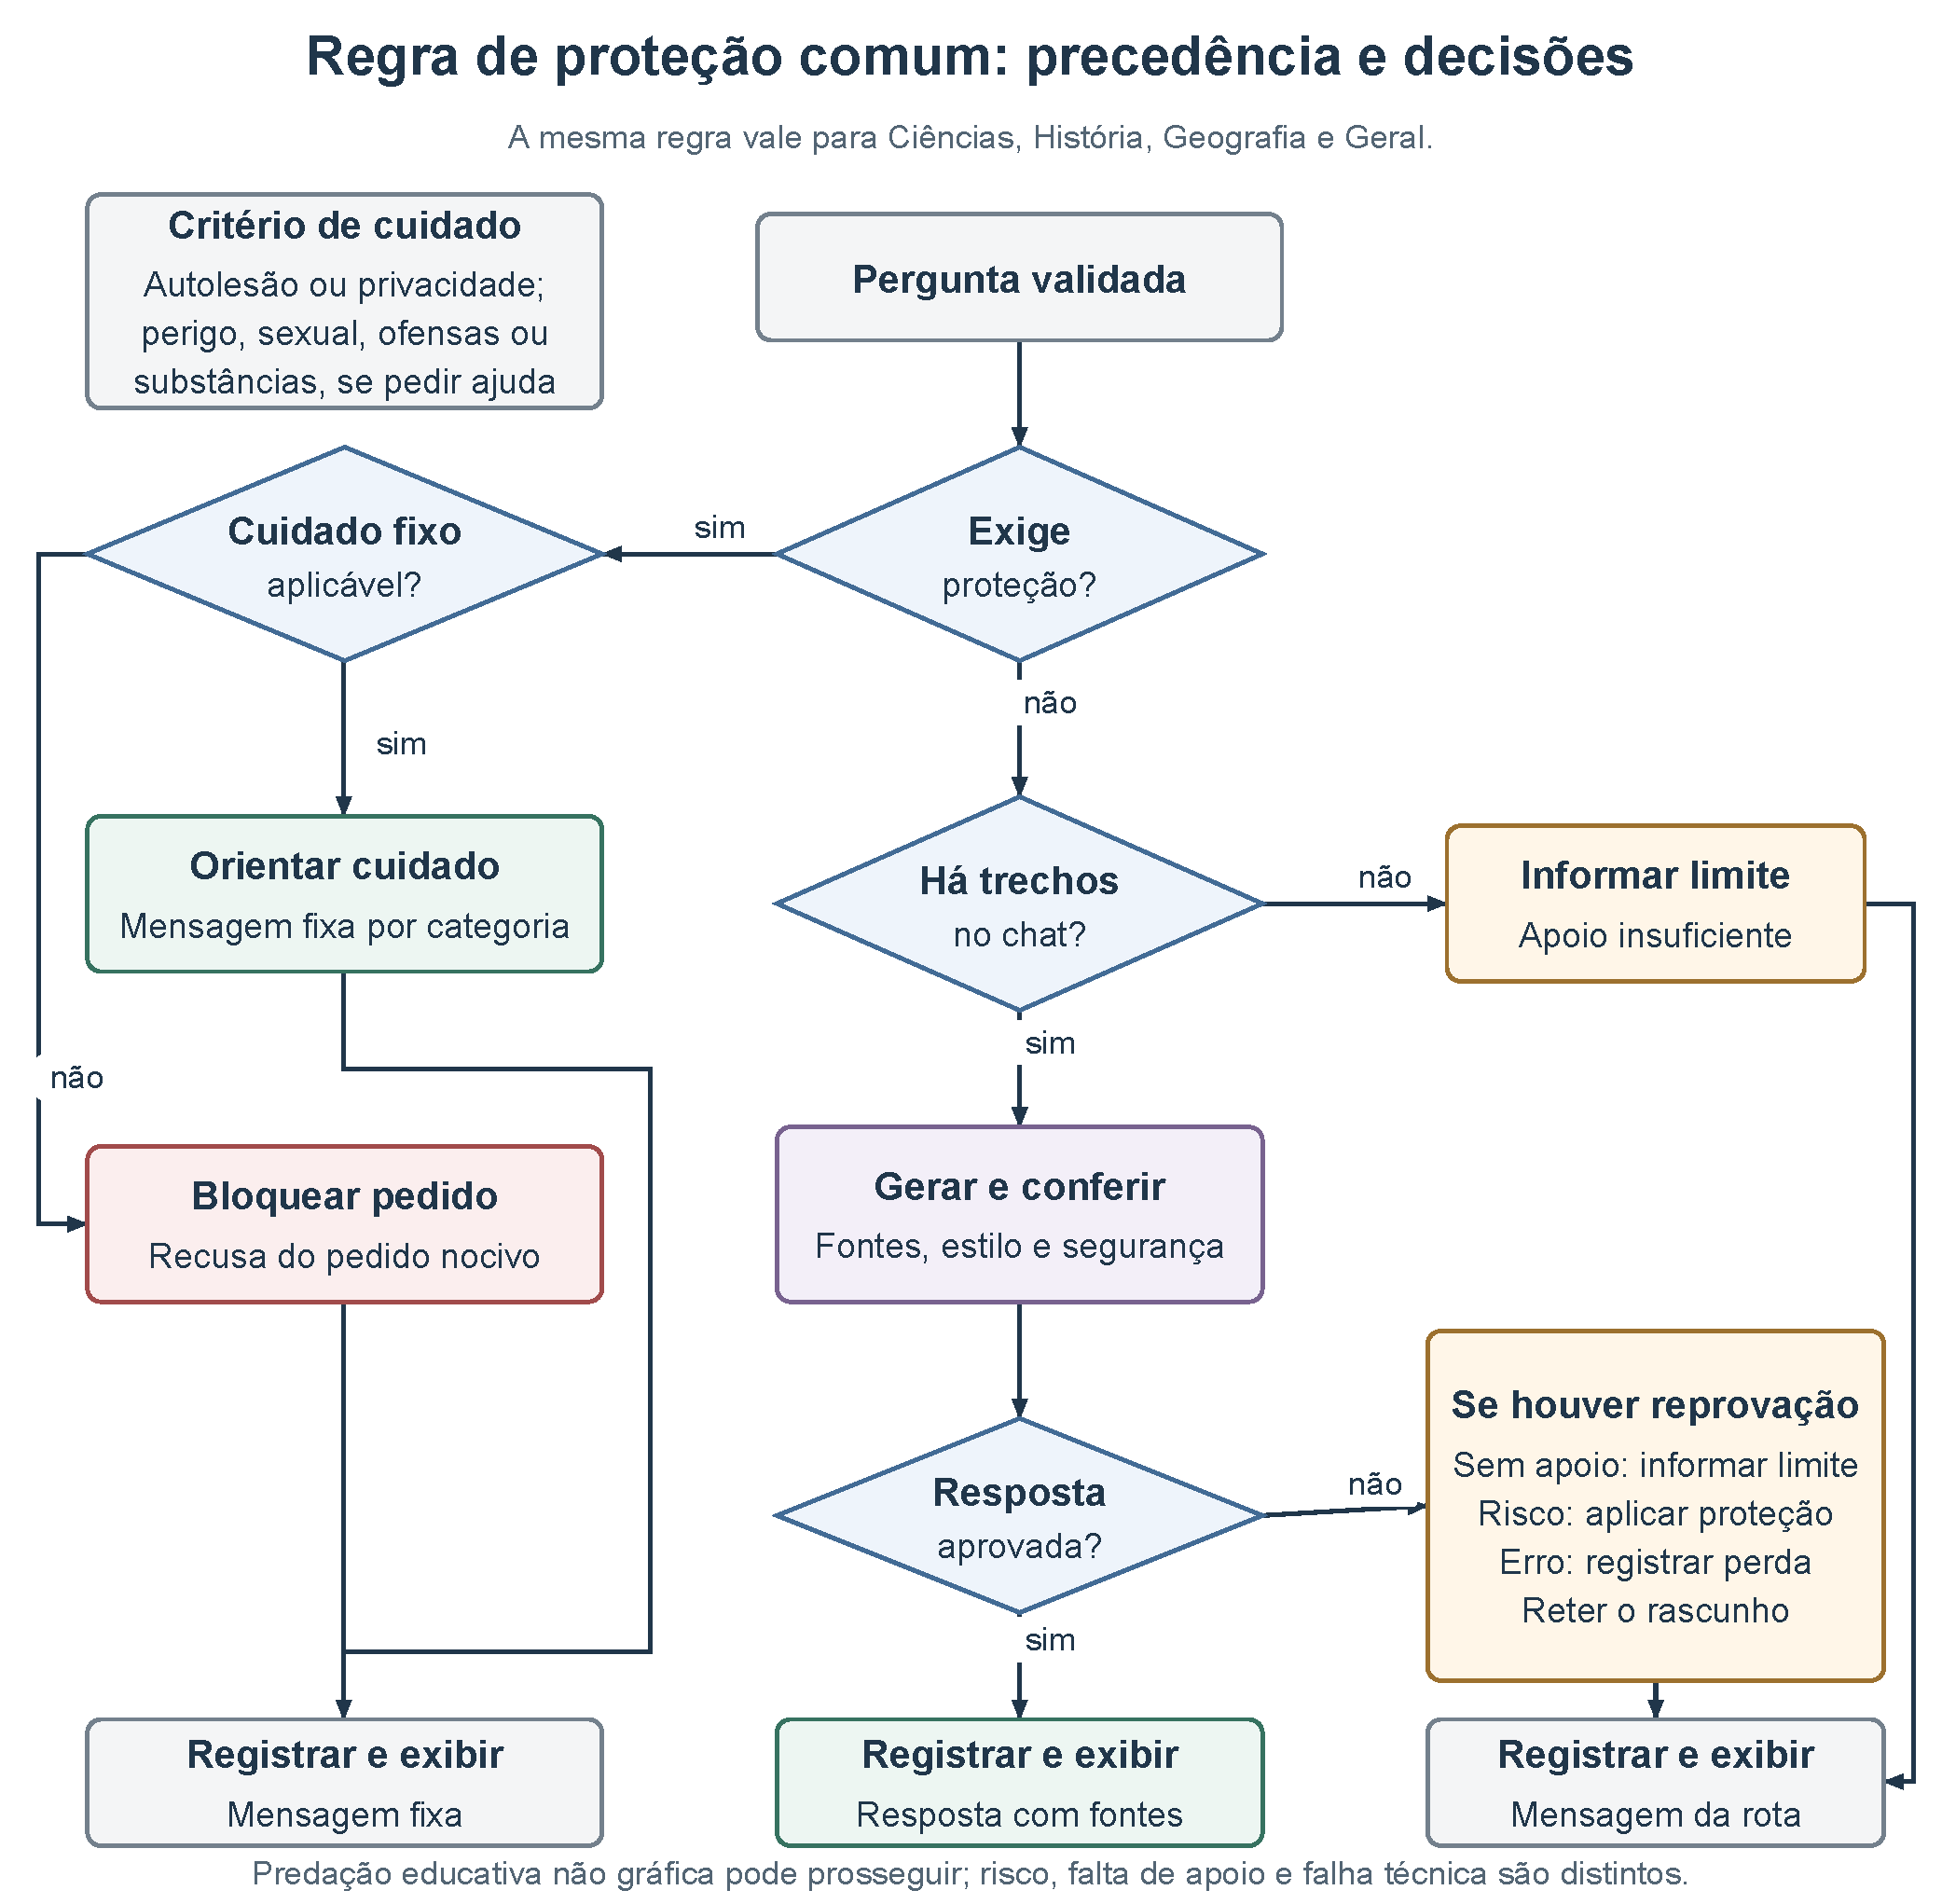
\includegraphics[width=\textwidth]{diagramas/pdf/07_regra_protecao_comum.pdf}

\caption{Precedência das decisões de entrada e saída}\label{fig:decisao}
\fonte{Elaboração própria; regras implementadas na função \texttt{decision}.}
\end{figure}

A Figura~\ref{fig:decisao} mostra a precedência da proteção. Uma explicação educativa de predação pode prosseguir se não exigir intervenção. A categoria de autolesão ou privacidade conduz à orientação; nas categorias perigo, sexual, ofensa e substância, a orientação depende também do reconhecimento de ajuda. Nos demais riscos, bloqueia-se. A configuração ativa não oferece uma condição que proíba predação educativa por si só.

\subsection{Pseudocódigos}

\begin{algorithm}[htbp]
\caption{Fluxo resumido da versão atual}\label{alg:fluxo}
\Entrada{pergunta, chat, estilo, regra comum e índice verificados}
\Saida{mensagem e registro, ou erro de persistência sem liberar resposta}
Validar entrada, exclusão mútua e orçamento temporal\;
Detectar identificadores localmente ou classificar entrada\;
Aplicar regra comum com precedência da proteção\;
\eSe{a rota inicial permite prosseguir}{
Filtrar o chat e recuperar até três passagens com limiar configurado\;
\eSe{não há passagens}{Definir redirecionamento\;}{
Gerar resposta estruturada no estilo escolhido\;
\eSe{o gerador declara insuficiência}{Definir redirecionamento\;}{
Validar resposta, extensão, citações e dados pessoais\;
Verificar sustentação semântica nas fontes citadas\;
\eSe{não sustentada}{Definir redirecionamento\;}{Classificar saída e aplicar proteção\;}
}}
}{Definir mensagem fixa de bloqueio ou orientação\;}
Em exceção técnica, registrar perda e mensagem de indisponibilidade\;
Persistir atomicamente; se falhar, reter a resposta e sinalizar erro\;
\end{algorithm}

O Algoritmo~\ref{alg:fluxo} distingue falha técnica de insuficiência e proteção. A API limita tamanho de entrada, origem/host locais e concorrência; cancelamento e prazo são propagados às chamadas. Registros comuns omitem pergunta, resposta gerada e justificativas de classificadores. Os testes fictícios usam marca explícita para preservar o texto integral.

Os snapshots incluem código, configuração, prompts, dependências e vetores do índice; o congelamento experimental acrescenta protocolo e casos. Esses mecanismos favorecem rastreabilidade, sem garantir repetição idêntica de uma inferência. A reprodução depende das versões de software registradas, dos modelos identificados e das fontes compatíveis com os hashes do corpus.
